% 66-44(66쪽) — 도함수 y=f'(x) 의 그래프(아래로 볼록한 포물선 · x축과 -1, 1 에서 만난다).
% 원문에 있는 것만: 곡선 · 라벨 y=f'(x), -1, O, 1, x, y. 꼭짓점 값 등 원문에 없는 눈금은 넣지 않는다.
% 스캔 화질이 낮아 TikZ 로 다시 그림.
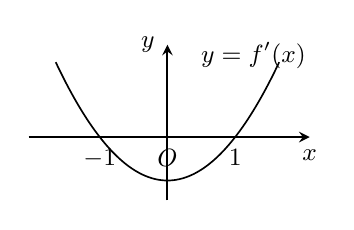
\begin{tikzpicture}[x=0.86cm, y=0.46cm, line width=0.5pt]
  \draw[->, >=stealth, line width=0.7pt] (-2.05,0) -- (2.10,0) node[below=1pt, font=\small] {$x$};
  \draw[->, >=stealth, line width=0.7pt] (0,-1.75) -- (0,2.55) node[left=1pt, font=\small] {$y$};
  \draw[line width=0.6pt, domain=-1.65:1.65, samples=110, smooth]
    plot (\x, {1.2*((\x)*(\x)-1)});
  \node[below=1pt, font=\small] at (-1,0) {$-1$};
  \node[below=1pt, font=\small] at (0,0) {$\pt{O}$};
  \node[below=1pt, font=\small] at (1,0) {$1$};
  \node[anchor=west, font=\small] at (0.35,2.25) {$y=f'(x)$};
\end{tikzpicture}
